\documentclass[1p]{elsarticle_modified}
%\bibliographystyle{elsarticle-num}

%\usepackage[colorlinks]{hyperref}
%\usepackage{abbrmath_seonhwa} %\Abb, \Ascr, \Acal ,\Abf, \Afrak
\usepackage{amsfonts}
\usepackage{amssymb}
\usepackage{amsmath}
\usepackage{amsthm}
\usepackage{scalefnt}
\usepackage{amsbsy}
\usepackage{kotex}
\usepackage{caption}
\usepackage{subfig}
\usepackage{color}
\usepackage{graphicx}
\usepackage{xcolor} %% white, black, red, green, blue, cyan, magenta, yellow
\usepackage{float}
\usepackage{setspace}
\usepackage{hyperref}

\usepackage{tikz}
\usetikzlibrary{arrows}

\usepackage{multirow}
\usepackage{array} % fixed length table
\usepackage{hhline}

%%%%%%%%%%%%%%%%%%%%%
\makeatletter
\renewcommand*\env@matrix[1][\arraystretch]{%
	\edef\arraystretch{#1}%
	\hskip -\arraycolsep
	\let\@ifnextchar\new@ifnextchar
	\array{*\c@MaxMatrixCols c}}
\makeatother %https://tex.stackexchange.com/questions/14071/how-can-i-increase-the-line-spacing-in-a-matrix
%%%%%%%%%%%%%%%

\usepackage[normalem]{ulem}

\newcommand{\msout}[1]{\ifmmode\text{\sout{\ensuremath{#1}}}\else\sout{#1}\fi}
%SOURCE: \msout is \stkout macro in https://tex.stackexchange.com/questions/20609/strikeout-in-math-mode

\newcommand{\cancel}[1]{
	\ifmmode
	{\color{red}\msout{#1}}
	\else
	{\color{red}\sout{#1}}
	\fi
}

\newcommand{\add}[1]{
	{\color{blue}\uwave{#1}}
}

\newcommand{\replace}[2]{
	\ifmmode
	{\color{red}\msout{#1}}{\color{blue}\uwave{#2}}
	\else
	{\color{red}\sout{#1}}{\color{blue}\uwave{#2}}
	\fi
}

\newcommand{\Sol}{\mathcal{S}} %segment
\newcommand{\D}{D} %diagram
\newcommand{\A}{\mathcal{A}} %arc


%%%%%%%%%%%%%%%%%%%%%%%%%%%%%5 test

\def\sl{\operatorname{\textup{SL}}(2,\Cbb)}
\def\psl{\operatorname{\textup{PSL}}(2,\Cbb)}
\def\quan{\mkern 1mu \triangleright \mkern 1mu}

\theoremstyle{definition}
\newtheorem{thm}{Theorem}[section]
\newtheorem{prop}[thm]{Proposition}
\newtheorem{lem}[thm]{Lemma}
\newtheorem{ques}[thm]{Question}
\newtheorem{cor}[thm]{Corollary}
\newtheorem{defn}[thm]{Definition}
\newtheorem{exam}[thm]{Example}
\newtheorem{rmk}[thm]{Remark}
\newtheorem{alg}[thm]{Algorithm}

\newcommand{\I}{\sqrt{-1}}
\begin{document}

%\begin{frontmatter}
%
%\title{Boundary parabolic representations of knots up to 8 crossings}
%
%%% Group authors per affiliation:
%\author{Yunhi Cho} 
%\address{Department of Mathematics, University of Seoul, Seoul, Korea}
%\ead{yhcho@uos.ac.kr}
%
%
%\author{Seonhwa Kim} %\fnref{s_kim}}
%\address{Center for Geometry and Physics, Institute for Basic Science, Pohang, 37673, Korea}
%\ead{ryeona17@ibs.re.kr}
%
%\author{Hyuk Kim}
%\address{Department of Mathematical Sciences, Seoul National University, Seoul 08826, Korea}
%\ead{hyukkim@snu.ac.kr}
%
%\author{Seokbeom Yoon}
%\address{Department of Mathematical Sciences, Seoul National University, Seoul, 08826,  Korea}
%\ead{sbyoon15@snu.ac.kr}
%
%\begin{abstract}
%We find all boundary parabolic representation of knots up to 8 crossings.
%
%\end{abstract}
%\begin{keyword}
%    \MSC[2010] 57M25 
%\end{keyword}
%
%\end{frontmatter}

%\linenumbers
%\tableofcontents
%
\newcommand\colored[1]{\textcolor{white}{\rule[-0.35ex]{0.8em}{1.4ex}}\kern-0.8em\color{red} #1}%
%\newcommand\colored[1]{\textcolor{white}{ #1}\kern-2.17ex	\textcolor{white}{ #1}\kern-1.81ex	\textcolor{white}{ #1}\kern-2.15ex\color{red}#1	}

{\Large $\underline{11a_{222}~(K11a_{222})}$}

\setlength{\tabcolsep}{10pt}
\renewcommand{\arraystretch}{1.6}
\vspace{1cm}\begin{tabular}{m{100pt}>{\centering\arraybackslash}m{274pt}}
\multirow{5}{120pt}{
	\centering
	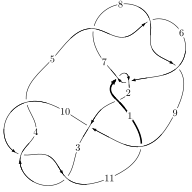
\includegraphics[width=112pt]{../../../GIT/diagram.site/Diagrams/png/471_11a_222.png}\\
\ \ \ A knot diagram\footnotemark}&
\allowdisplaybreaks
\textbf{Linearized knot diagam} \\
\cline{2-2}
 &
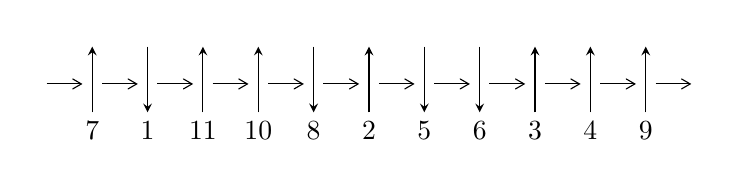
\begin{tikzpicture}[x=20pt, y=17pt]
	% nodes
	\node (C0) at (0, 0) {};
	\node (C1) at (1, 0) {};
	\node (C1U) at (1, +1) {};
	\node (C1D) at (1, -1) {7};

	\node (C2) at (2, 0) {};
	\node (C2U) at (2, +1) {};
	\node (C2D) at (2, -1) {1};

	\node (C3) at (3, 0) {};
	\node (C3U) at (3, +1) {};
	\node (C3D) at (3, -1) {11};

	\node (C4) at (4, 0) {};
	\node (C4U) at (4, +1) {};
	\node (C4D) at (4, -1) {10};

	\node (C5) at (5, 0) {};
	\node (C5U) at (5, +1) {};
	\node (C5D) at (5, -1) {8};

	\node (C6) at (6, 0) {};
	\node (C6U) at (6, +1) {};
	\node (C6D) at (6, -1) {2};

	\node (C7) at (7, 0) {};
	\node (C7U) at (7, +1) {};
	\node (C7D) at (7, -1) {5};

	\node (C8) at (8, 0) {};
	\node (C8U) at (8, +1) {};
	\node (C8D) at (8, -1) {6};

	\node (C9) at (9, 0) {};
	\node (C9U) at (9, +1) {};
	\node (C9D) at (9, -1) {3};

	\node (C10) at (10, 0) {};
	\node (C10U) at (10, +1) {};
	\node (C10D) at (10, -1) {4};

	\node (C11) at (11, 0) {};
	\node (C11U) at (11, +1) {};
	\node (C11D) at (11, -1) {9};
	\node (C12) at (12, 0) {};

	% arrows
	\draw[->,>={angle 60}]
	(C0) edge (C1) (C1) edge (C2) (C2) edge (C3) (C3) edge (C4) (C4) edge (C5) (C5) edge (C6) (C6) edge (C7) (C7) edge (C8) (C8) edge (C9) (C9) edge (C10) (C10) edge (C11) (C11) edge (C12) ;	\draw[->,>=stealth]
	(C1D) edge (C1U) (C2U) edge (C2D) (C3D) edge (C3U) (C4D) edge (C4U) (C5U) edge (C5D) (C6D) edge (C6U) (C7U) edge (C7D) (C8U) edge (C8D) (C9D) edge (C9U) (C10D) edge (C10U) (C11D) edge (C11U) ;
	\end{tikzpicture} \\
\hhline{~~} \\& 
\textbf{Solving Sequence} \\ \cline{2-2} 
 &
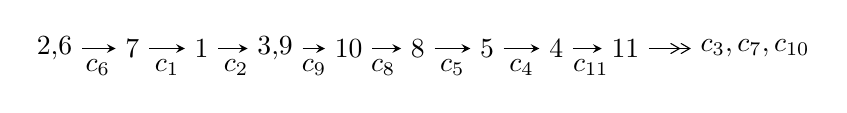
\begin{tikzpicture}[x=25pt, y=7pt]
	% node
	\node (A0) at (-1/8, 0) {2,6};
	\node (A1) at (1, 0) {7};
	\node (A2) at (2, 0) {1};
	\node (A3) at (49/16, 0) {3,9};
	\node (A4) at (33/8, 0) {10};
	\node (A5) at (41/8, 0) {8};
	\node (A6) at (49/8, 0) {5};
	\node (A7) at (57/8, 0) {4};
	\node (A8) at (65/8, 0) {11};
	\node (C1) at (1/2, -1) {$c_{6}$};
	\node (C2) at (3/2, -1) {$c_{1}$};
	\node (C3) at (5/2, -1) {$c_{2}$};
	\node (C4) at (29/8, -1) {$c_{9}$};
	\node (C5) at (37/8, -1) {$c_{8}$};
	\node (C6) at (45/8, -1) {$c_{5}$};
	\node (C7) at (53/8, -1) {$c_{4}$};
	\node (C8) at (61/8, -1) {$c_{11}$};
	\node (A9) at (10, 0) {$c_{3},c_{7},c_{10}$};

	% edge
	\draw[->,>=stealth]	
	(A0) edge (A1) (A1) edge (A2) (A2) edge (A3) (A3) edge (A4) (A4) edge (A5) (A5) edge (A6) (A6) edge (A7) (A7) edge (A8) ;
	\draw[->>,>={angle 60}]	
	(A8) edge (A9);
\end{tikzpicture} \\ 

\end{tabular} \\

\footnotetext{
The image of knot diagram is generated by the software ``\textbf{Draw programme}" developed by Andrew Bartholomew(\url{http://www.layer8.co.uk/maths/draw/index.htm\#Running-draw}), where we modified some parts for our purpose(\url{https://github.com/CATsTAILs/LinksPainter}).
}\phantom \\ \newline 
\centering \textbf{Ideals for irreducible components\footnotemark of $X_{\text{par}}$} 
 
\begin{align*}
I^u_{1}&=\langle 
-3.72396\times10^{40} u^{52}-2.67316\times10^{41} u^{51}+\cdots+2.67330\times10^{41} b+1.99338\times10^{42},\\
\phantom{I^u_{1}}&\phantom{= \langle  }4.74949\times10^{40} u^{52}+1.41444\times10^{41} u^{51}+\cdots+1.06932\times10^{42} a-1.40219\times10^{42},\;u^{53}+u^{52}+\cdots-12 u-8\rangle \\
\\
I^v_{1}&=\langle 
a,\;b-1,\;v^3+v^2-1\rangle \\
\end{align*}
\raggedright * 2 irreducible components of $\dim_{\mathbb{C}}=0$, with total 56 representations.\\
\footnotetext{All coefficients of polynomials are rational numbers. But the coefficients are sometimes approximated in decimal forms when there is not enough margin.}
\newpage
\renewcommand{\arraystretch}{1}
\centering \section*{I. $I^u_{1}= \langle -3.72\times10^{40} u^{52}-2.67\times10^{41} u^{51}+\cdots+2.67\times10^{41} b+1.99\times10^{42},\;4.75\times10^{40} u^{52}+1.41\times10^{41} u^{51}+\cdots+1.07\times10^{42} a-1.40\times10^{42},\;u^{53}+u^{52}+\cdots-12 u-8 \rangle$}
\flushleft \textbf{(i) Arc colorings}\\
\begin{tabular}{m{7pt} m{180pt} m{7pt} m{180pt} }
\flushright $a_{2}=$&$\begin{pmatrix}0\\u\end{pmatrix}$ \\
\flushright $a_{6}=$&$\begin{pmatrix}1\\0\end{pmatrix}$ \\
\flushright $a_{7}=$&$\begin{pmatrix}1\\- u^2\end{pmatrix}$ \\
\flushright $a_{1}=$&$\begin{pmatrix}- u\\u^3+u\end{pmatrix}$ \\
\flushright $a_{3}=$&$\begin{pmatrix}- u^3\\u^5+u^3+u\end{pmatrix}$ \\
\flushright $a_{9}=$&$\begin{pmatrix}-0.0444159 u^{52}-0.132274 u^{51}+\cdots+1.64666 u+1.31129\\0.139302 u^{52}+0.999947 u^{51}+\cdots-7.49767 u-7.45663\end{pmatrix}$ \\
\flushright $a_{10}=$&$\begin{pmatrix}-0.343615 u^{52}+0.405811 u^{51}+\cdots-0.582641 u-2.59994\\0.279844 u^{52}+1.23840 u^{51}+\cdots-9.65395 u-10.2736\end{pmatrix}$ \\
\flushright $a_{8}=$&$\begin{pmatrix}0.0948858 u^{52}+0.867673 u^{51}+\cdots-5.85102 u-6.14534\\0.139302 u^{52}+0.999947 u^{51}+\cdots-7.49767 u-7.45663\end{pmatrix}$ \\
\flushright $a_{5}=$&$\begin{pmatrix}0.0948858 u^{52}+0.867673 u^{51}+\cdots-5.85102 u-6.14534\\0.275865 u^{52}-0.199028 u^{51}+\cdots-2.53486 u+1.27433\end{pmatrix}$ \\
\flushright $a_{4}=$&$\begin{pmatrix}-1.49188 u^{52}-0.252221 u^{51}+\cdots+12.9241 u+1.42483\\-0.260130 u^{52}-0.116987 u^{51}+\cdots+1.92031 u-1.17979\end{pmatrix}$ \\
\flushright $a_{11}=$&$\begin{pmatrix}0.424578 u^{52}+0.931561 u^{51}+\cdots-9.23571 u-8.47524\\0.273370 u^{52}+0.479526 u^{51}+\cdots-2.54983 u-4.25728\end{pmatrix}$\\ \flushright $a_{11}=$&$\begin{pmatrix}0.424578 u^{52}+0.931561 u^{51}+\cdots-9.23571 u-8.47524\\0.273370 u^{52}+0.479526 u^{51}+\cdots-2.54983 u-4.25728\end{pmatrix}$\\&\end{tabular}
\flushleft \textbf{(ii) Obstruction class $= -1$}\\~\\
\flushleft \textbf{(iii) Cusp Shapes $= -0.353691 u^{52}-0.908611 u^{51}+\cdots+0.108906 u+7.17724$}\\~\\
\newpage\renewcommand{\arraystretch}{1}
\flushleft \textbf{(iv) u-Polynomials at the component}\newline \\
\begin{tabular}{m{50pt}|m{274pt}}
Crossings & \hspace{64pt}u-Polynomials at each crossing \\
\hline $$\begin{aligned}c_{1},c_{6}\end{aligned}$$&$\begin{aligned}
&u^{53}+u^{52}+\cdots-12 u-8
\end{aligned}$\\
\hline $$\begin{aligned}c_{2}\end{aligned}$$&$\begin{aligned}
&u^{53}+21 u^{52}+\cdots-112 u-64
\end{aligned}$\\
\hline $$\begin{aligned}c_{3},c_{4},c_{10}\end{aligned}$$&$\begin{aligned}
&u^{53}+2 u^{52}+\cdots-3 u-1
\end{aligned}$\\
\hline $$\begin{aligned}c_{5},c_{7},c_{8}\end{aligned}$$&$\begin{aligned}
&u^{53}-4 u^{52}+\cdots+6 u-1
\end{aligned}$\\
\hline $$\begin{aligned}c_{9}\end{aligned}$$&$\begin{aligned}
&u^{53}-2 u^{52}+\cdots-3 u-1
\end{aligned}$\\
\hline $$\begin{aligned}c_{11}\end{aligned}$$&$\begin{aligned}
&u^{53}+12 u^{52}+\cdots-1235 u-131
\end{aligned}$\\
\hline
\end{tabular}\\~\\
\newpage\renewcommand{\arraystretch}{1}
\flushleft \textbf{(v) Riley Polynomials at the component}\newline \\
\begin{tabular}{m{50pt}|m{274pt}}
Crossings & \hspace{64pt}Riley Polynomials at each crossing \\
\hline $$\begin{aligned}c_{1},c_{6}\end{aligned}$$&$\begin{aligned}
&y^{53}+21 y^{52}+\cdots-112 y-64
\end{aligned}$\\
\hline $$\begin{aligned}c_{2}\end{aligned}$$&$\begin{aligned}
&y^{53}+17 y^{52}+\cdots+167168 y-4096
\end{aligned}$\\
\hline $$\begin{aligned}c_{3},c_{4},c_{10}\end{aligned}$$&$\begin{aligned}
&y^{53}+48 y^{52}+\cdots+y-1
\end{aligned}$\\
\hline $$\begin{aligned}c_{5},c_{7},c_{8}\end{aligned}$$&$\begin{aligned}
&y^{53}-46 y^{52}+\cdots+38 y-1
\end{aligned}$\\
\hline $$\begin{aligned}c_{9}\end{aligned}$$&$\begin{aligned}
&y^{53}+54 y^{51}+\cdots+y-1
\end{aligned}$\\
\hline $$\begin{aligned}c_{11}\end{aligned}$$&$\begin{aligned}
&y^{53}+12 y^{52}+\cdots-263187 y-17161
\end{aligned}$\\
\hline
\end{tabular}\\~\\
\newpage\flushleft \textbf{(vi) Complex Volumes and Cusp Shapes}
$$\begin{array}{c|c|c}  
\text{Solutions to }I^u_{1}& \I (\text{vol} + \sqrt{-1}CS) & \text{Cusp shape}\\
 \hline 
\begin{aligned}
u &= \phantom{-}0.098959 + 0.985230 I \\
a &= -0.216031 - 0.691134 I \\
b &= \phantom{-}0.741431 + 0.530945 I\end{aligned}
 & -6.86405 - 3.34890 I & -5.53237 + 3.71045 I \\ \hline\begin{aligned}
u &= \phantom{-}0.098959 - 0.985230 I \\
a &= -0.216031 + 0.691134 I \\
b &= \phantom{-}0.741431 - 0.530945 I\end{aligned}
 & -6.86405 + 3.34890 I & -5.53237 - 3.71045 I \\ \hline\begin{aligned}
u &= \phantom{-}0.484801 + 0.904145 I \\
a &= -0.86642 - 2.04538 I \\
b &= -1.271870 + 0.230719 I\end{aligned}
 & -0.82302 + 2.29845 I & \phantom{-}2.07591 - 2.82759 I \\ \hline\begin{aligned}
u &= \phantom{-}0.484801 - 0.904145 I \\
a &= -0.86642 + 2.04538 I \\
b &= -1.271870 - 0.230719 I\end{aligned}
 & -0.82302 - 2.29845 I & \phantom{-}2.07591 + 2.82759 I \\ \hline\begin{aligned}
u &= \phantom{-}0.665810 + 0.798402 I \\
a &= \phantom{-}0.568425 + 1.140550 I \\
b &= \phantom{-}0.077045 - 0.713159 I\end{aligned}
 & \phantom{-}0.59121 + 2.50996 I & \phantom{-}4.33610 - 3.95071 I \\ \hline\begin{aligned}
u &= \phantom{-}0.665810 - 0.798402 I \\
a &= \phantom{-}0.568425 - 1.140550 I \\
b &= \phantom{-}0.077045 + 0.713159 I\end{aligned}
 & \phantom{-}0.59121 - 2.50996 I & \phantom{-}4.33610 + 3.95071 I \\ \hline\begin{aligned}
u &= -0.704489 + 0.647178 I \\
a &= \phantom{-}0.750323 - 1.123850 I \\
b &= -0.034455 + 0.645365 I\end{aligned}
 & \phantom{-}2.99577 + 0.83630 I & \phantom{-}8.46469 - 1.37155 I \\ \hline\begin{aligned}
u &= -0.704489 - 0.647178 I \\
a &= \phantom{-}0.750323 + 1.123850 I \\
b &= -0.034455 - 0.645365 I\end{aligned}
 & \phantom{-}2.99577 - 0.83630 I & \phantom{-}8.46469 + 1.37155 I \\ \hline\begin{aligned}
u &= -0.701831 + 0.644298 I \\
a &= -0.707620 + 0.370746 I \\
b &= \phantom{-}1.161210 - 0.306433 I\end{aligned}
 & -2.68045 + 1.19639 I & \phantom{-}0.561902 - 0.388264 I \\ \hline\begin{aligned}
u &= -0.701831 - 0.644298 I \\
a &= -0.707620 - 0.370746 I \\
b &= \phantom{-}1.161210 + 0.306433 I\end{aligned}
 & -2.68045 - 1.19639 I & \phantom{-}0.561902 + 0.388264 I\\
 \hline 
 \end{array}$$\newpage$$\begin{array}{c|c|c}  
\text{Solutions to }I^u_{1}& \I (\text{vol} + \sqrt{-1}CS) & \text{Cusp shape}\\
 \hline 
\begin{aligned}
u &= -0.438735 + 0.954883 I \\
a &= -0.519557 + 0.602280 I \\
b &= \phantom{-}0.993065 - 0.486660 I\end{aligned}
 & -5.75404 - 4.81132 I & -3.33331 + 4.06462 I \\ \hline\begin{aligned}
u &= -0.438735 - 0.954883 I \\
a &= -0.519557 - 0.602280 I \\
b &= \phantom{-}0.993065 + 0.486660 I\end{aligned}
 & -5.75404 + 4.81132 I & -3.33331 - 4.06462 I \\ \hline\begin{aligned}
u &= \phantom{-}0.456523 + 0.829696 I \\
a &= -0.527363 - 0.500478 I \\
b &= \phantom{-}1.006360 + 0.404023 I\end{aligned}
 & -0.53651 + 1.57348 I & \phantom{-}1.80074 - 4.58385 I \\ \hline\begin{aligned}
u &= \phantom{-}0.456523 - 0.829696 I \\
a &= -0.527363 + 0.500478 I \\
b &= \phantom{-}1.006360 - 0.404023 I\end{aligned}
 & -0.53651 - 1.57348 I & \phantom{-}1.80074 + 4.58385 I \\ \hline\begin{aligned}
u &= \phantom{-}0.576999 + 0.889147 I \\
a &= \phantom{-}0.435650 + 1.098150 I \\
b &= \phantom{-}0.180982 - 0.721453 I\end{aligned}
 & \phantom{-}0.38779 + 2.33704 I & \phantom{-}2.43384 - 2.57524 I \\ \hline\begin{aligned}
u &= \phantom{-}0.576999 - 0.889147 I \\
a &= \phantom{-}0.435650 - 1.098150 I \\
b &= \phantom{-}0.180982 + 0.721453 I\end{aligned}
 & \phantom{-}0.38779 - 2.33704 I & \phantom{-}2.43384 + 2.57524 I \\ \hline\begin{aligned}
u &= \phantom{-}0.753024 + 0.562381 I \\
a &= \phantom{-}0.86895 + 1.15997 I \\
b &= -0.115897 - 0.626414 I\end{aligned}
 & -1.92655 - 4.26986 I & \phantom{-}3.38600 + 2.83654 I \\ \hline\begin{aligned}
u &= \phantom{-}0.753024 - 0.562381 I \\
a &= \phantom{-}0.86895 - 1.15997 I \\
b &= -0.115897 + 0.626414 I\end{aligned}
 & -1.92655 + 4.26986 I & \phantom{-}3.38600 - 2.83654 I \\ \hline\begin{aligned}
u &= \phantom{-}1.030490 + 0.261952 I \\
a &= -0.910866 - 0.146722 I \\
b &= \phantom{-}1.337480 + 0.124077 I\end{aligned}
 & -8.23681 + 0.97965 I & -4.65901 - 0.74482 I \\ \hline\begin{aligned}
u &= \phantom{-}1.030490 - 0.261952 I \\
a &= -0.910866 + 0.146722 I \\
b &= \phantom{-}1.337480 - 0.124077 I\end{aligned}
 & -8.23681 - 0.97965 I & -4.65901 + 0.74482 I\\
 \hline 
 \end{array}$$\newpage$$\begin{array}{c|c|c}  
\text{Solutions to }I^u_{1}& \I (\text{vol} + \sqrt{-1}CS) & \text{Cusp shape}\\
 \hline 
\begin{aligned}
u &= -0.388639 + 0.850959 I \\
a &= -1.37535 + 2.10142 I \\
b &= -1.248240 - 0.181646 I\end{aligned}
 & -5.29869 + 1.45751 I & -3.56392 + 1.11425 I \\ \hline\begin{aligned}
u &= -0.388639 - 0.850959 I \\
a &= -1.37535 - 2.10142 I \\
b &= -1.248240 + 0.181646 I\end{aligned}
 & -5.29869 - 1.45751 I & -3.56392 - 1.11425 I \\ \hline\begin{aligned}
u &= -0.412964 + 1.005730 I \\
a &= \phantom{-}0.231844 - 1.026890 I \\
b &= \phantom{-}0.346311 + 0.718386 I\end{aligned}
 & -5.68668 - 1.06282 I & -2.80690 + 2.95348 I \\ \hline\begin{aligned}
u &= -0.412964 - 1.005730 I \\
a &= \phantom{-}0.231844 + 1.026890 I \\
b &= \phantom{-}0.346311 - 0.718386 I\end{aligned}
 & -5.68668 + 1.06282 I & -2.80690 - 2.95348 I \\ \hline\begin{aligned}
u &= \phantom{-}0.961697 + 0.529123 I \\
a &= -0.870380 - 0.301578 I \\
b &= \phantom{-}1.299930 + 0.254117 I\end{aligned}
 & -1.18376 - 4.09953 I & \phantom{-}2.32118 + 4.98239 I \\ \hline\begin{aligned}
u &= \phantom{-}0.961697 - 0.529123 I \\
a &= -0.870380 + 0.301578 I \\
b &= \phantom{-}1.299930 - 0.254117 I\end{aligned}
 & -1.18376 + 4.09953 I & \phantom{-}2.32118 - 4.98239 I \\ \hline\begin{aligned}
u &= -0.815444 + 0.371656 I \\
a &= -0.786076 + 0.206543 I \\
b &= \phantom{-}1.231550 - 0.172173 I\end{aligned}
 & -2.47497 + 0.74735 I & -0.90212 + 1.24909 I \\ \hline\begin{aligned}
u &= -0.815444 - 0.371656 I \\
a &= -0.786076 - 0.206543 I \\
b &= \phantom{-}1.231550 + 0.172173 I\end{aligned}
 & -2.47497 - 0.74735 I & -0.90212 - 1.24909 I \\ \hline\begin{aligned}
u &= -0.580487 + 0.976562 I \\
a &= -0.46963 + 1.90355 I \\
b &= -1.306780 - 0.280326 I\end{aligned}
 & -3.72441 - 6.08956 I & -1.10463 + 6.46640 I \\ \hline\begin{aligned}
u &= -0.580487 - 0.976562 I \\
a &= -0.46963 - 1.90355 I \\
b &= -1.306780 + 0.280326 I\end{aligned}
 & -3.72441 + 6.08956 I & -1.10463 - 6.46640 I\\
 \hline 
 \end{array}$$\newpage$$\begin{array}{c|c|c}  
\text{Solutions to }I^u_{1}& \I (\text{vol} + \sqrt{-1}CS) & \text{Cusp shape}\\
 \hline 
\begin{aligned}
u &= -1.041700 + 0.533025 I \\
a &= -0.917846 + 0.303340 I \\
b &= \phantom{-}1.340090 - 0.256972 I\end{aligned}
 & -6.53406 + 7.50813 I & -2.48060 - 5.10060 I \\ \hline\begin{aligned}
u &= -1.041700 - 0.533025 I \\
a &= -0.917846 - 0.303340 I \\
b &= \phantom{-}1.340090 + 0.256972 I\end{aligned}
 & -6.53406 - 7.50813 I & -2.48060 + 5.10060 I \\ \hline\begin{aligned}
u &= -0.633586 + 0.994698 I \\
a &= \phantom{-}0.371306 - 1.203140 I \\
b &= \phantom{-}0.199005 + 0.815326 I\end{aligned}
 & \phantom{-}1.93858 - 5.99540 I & \phantom{-}5.14118 + 7.31361 I \\ \hline\begin{aligned}
u &= -0.633586 - 0.994698 I \\
a &= \phantom{-}0.371306 + 1.203140 I \\
b &= \phantom{-}0.199005 - 0.815326 I\end{aligned}
 & \phantom{-}1.93858 + 5.99540 I & \phantom{-}5.14118 - 7.31361 I \\ \hline\begin{aligned}
u &= -0.053370 + 0.778256 I \\
a &= -0.099463 + 0.457828 I \\
b &= \phantom{-}0.673274 - 0.340918 I\end{aligned}
 & -1.43718 + 1.12513 I & -2.70988 - 5.24060 I \\ \hline\begin{aligned}
u &= -0.053370 - 0.778256 I \\
a &= -0.099463 - 0.457828 I \\
b &= \phantom{-}0.673274 + 0.340918 I\end{aligned}
 & -1.43718 - 1.12513 I & -2.70988 + 5.24060 I \\ \hline\begin{aligned}
u &= \phantom{-}0.634803 + 1.049780 I \\
a &= \phantom{-}0.326864 + 1.231490 I \\
b &= \phantom{-}0.224599 - 0.849112 I\end{aligned}
 & -3.39969 + 9.56118 I & \phantom{-0.000000 } 0. - 7.56251 I \\ \hline\begin{aligned}
u &= \phantom{-}0.634803 - 1.049780 I \\
a &= \phantom{-}0.326864 - 1.231490 I \\
b &= \phantom{-}0.224599 + 0.849112 I\end{aligned}
 & -3.39969 - 9.56118 I & \phantom{-0.000000 -}0. + 7.56251 I \\ \hline\begin{aligned}
u &= -0.061506 + 1.244360 I \\
a &= -0.819931 + 0.179681 I \\
b &= -1.44045 - 0.02930 I\end{aligned}
 & -8.22882 - 1.96670 I & -4.21460 + 3.59094 I \\ \hline\begin{aligned}
u &= -0.061506 - 1.244360 I \\
a &= -0.819931 - 0.179681 I \\
b &= -1.44045 + 0.02930 I\end{aligned}
 & -8.22882 + 1.96670 I & -4.21460 - 3.59094 I\\
 \hline 
 \end{array}$$\newpage$$\begin{array}{c|c|c}  
\text{Solutions to }I^u_{1}& \I (\text{vol} + \sqrt{-1}CS) & \text{Cusp shape}\\
 \hline 
\begin{aligned}
u &= -0.630774 + 1.106670 I \\
a &= -0.22899 + 1.62310 I \\
b &= -1.372550 - 0.306311 I\end{aligned}
 & -4.53517 - 6.09494 I & \phantom{-0.000000 } 0 \\ \hline\begin{aligned}
u &= -0.630774 - 1.106670 I \\
a &= -0.22899 - 1.62310 I \\
b &= -1.372550 + 0.306311 I\end{aligned}
 & -4.53517 + 6.09494 I & \phantom{-0.000000 } 0 \\ \hline\begin{aligned}
u &= \phantom{-}0.564987 + 1.202570 I \\
a &= -0.252964 - 1.360110 I \\
b &= -1.42026 + 0.27304 I\end{aligned}
 & -11.29940 + 4.62469 I & \phantom{-0.000000 } 0 \\ \hline\begin{aligned}
u &= \phantom{-}0.564987 - 1.202570 I \\
a &= -0.252964 + 1.360110 I \\
b &= -1.42026 - 0.27304 I\end{aligned}
 & -11.29940 - 4.62469 I & \phantom{-0.000000 } 0 \\ \hline\begin{aligned}
u &= \phantom{-}0.698514 + 1.133990 I \\
a &= -0.07006 - 1.62273 I \\
b &= -1.38677 + 0.34044 I\end{aligned}
 & -3.08458 + 10.16490 I & \phantom{-0.000000 } 0 \\ \hline\begin{aligned}
u &= \phantom{-}0.698514 - 1.133990 I \\
a &= -0.07006 + 1.62273 I \\
b &= -1.38677 - 0.34044 I\end{aligned}
 & -3.08458 - 10.16490 I & \phantom{-0.000000 } 0 \\ \hline\begin{aligned}
u &= \phantom{-}0.109910 + 1.333410 I \\
a &= -0.563705 - 0.274434 I \\
b &= -1.48292 + 0.05239 I\end{aligned}
 & -14.2996 + 4.8556 I & \phantom{-0.000000 } 0 \\ \hline\begin{aligned}
u &= \phantom{-}0.109910 - 1.333410 I \\
a &= -0.563705 + 0.274434 I \\
b &= -1.48292 - 0.05239 I\end{aligned}
 & -14.2996 - 4.8556 I & \phantom{-0.000000 } 0 \\ \hline\begin{aligned}
u &= -0.723673 + 1.167980 I \\
a &= \phantom{-}0.00012 + 1.57826 I \\
b &= -1.40426 - 0.35282 I\end{aligned}
 & -8.5679 - 13.8903 I & \phantom{-0.000000 } 0 \\ \hline\begin{aligned}
u &= -0.723673 - 1.167980 I \\
a &= \phantom{-}0.00012 - 1.57826 I \\
b &= -1.40426 + 0.35282 I\end{aligned}
 & -8.5679 + 13.8903 I & \phantom{-0.000000 } 0\\
 \hline 
 \end{array}$$\newpage$$\begin{array}{c|c|c}  
\text{Solutions to }I^u_{1}& \I (\text{vol} + \sqrt{-1}CS) & \text{Cusp shape}\\
 \hline 
\begin{aligned}
u &= -0.546347 + 0.172932 I \\
a &= \phantom{-}1.47434 - 0.57598 I \\
b &= -0.248192 + 0.218926 I\end{aligned}
 & -3.39404 - 2.40292 I & \phantom{-}4.22803 + 2.59091 I \\ \hline\begin{aligned}
u &= -0.546347 - 0.172932 I \\
a &= \phantom{-}1.47434 + 0.57598 I \\
b &= -0.248192 - 0.218926 I\end{aligned}
 & -3.39404 + 2.40292 I & \phantom{-}4.22803 - 2.59091 I \\ \hline\begin{aligned}
u &= \phantom{-}0.394055\phantom{ +0.000000I} \\
a &= \phantom{-}1.34884\phantom{ +0.000000I} \\
b &= -0.159324\phantom{ +0.000000I}\end{aligned}
 & \phantom{-}0.852216\phantom{ +0.000000I} & \phantom{-}12.0640\phantom{ +0.000000I}\\
 \hline 
 \end{array}$$\newpage\newpage\renewcommand{\arraystretch}{1}
\centering \section*{II. $I^v_{1}= \langle a,\;b-1,\;v^3+v^2-1 \rangle$}
\flushleft \textbf{(i) Arc colorings}\\
\begin{tabular}{m{7pt} m{180pt} m{7pt} m{180pt} }
\flushright $a_{2}=$&$\begin{pmatrix}v\\0\end{pmatrix}$ \\
\flushright $a_{6}=$&$\begin{pmatrix}1\\0\end{pmatrix}$ \\
\flushright $a_{7}=$&$\begin{pmatrix}1\\0\end{pmatrix}$ \\
\flushright $a_{1}=$&$\begin{pmatrix}v\\0\end{pmatrix}$ \\
\flushright $a_{3}=$&$\begin{pmatrix}v\\0\end{pmatrix}$ \\
\flushright $a_{9}=$&$\begin{pmatrix}0\\1\end{pmatrix}$ \\
\flushright $a_{10}=$&$\begin{pmatrix}v^2\\1\end{pmatrix}$ \\
\flushright $a_{8}=$&$\begin{pmatrix}1\\1\end{pmatrix}$ \\
\flushright $a_{5}=$&$\begin{pmatrix}0\\-1\end{pmatrix}$ \\
\flushright $a_{4}=$&$\begin{pmatrix}v^2+v-1\\v^2-1\end{pmatrix}$ \\
\flushright $a_{11}=$&$\begin{pmatrix}v\\v\end{pmatrix}$\\ \flushright $a_{11}=$&$\begin{pmatrix}v\\v\end{pmatrix}$\\&\end{tabular}
\flushleft \textbf{(ii) Obstruction class $= 1$}\\~\\
\flushleft \textbf{(iii) Cusp Shapes $= - v^2+3 v+1$}\\~\\
\newpage\renewcommand{\arraystretch}{1}
\flushleft \textbf{(iv) u-Polynomials at the component}\newline \\
\begin{tabular}{m{50pt}|m{274pt}}
Crossings & \hspace{64pt}u-Polynomials at each crossing \\
\hline $$\begin{aligned}c_{1},c_{2},c_{6}\end{aligned}$$&$\begin{aligned}
&u^3
\end{aligned}$\\
\hline $$\begin{aligned}c_{3},c_{4}\end{aligned}$$&$\begin{aligned}
&u^3- u^2+2 u-1
\end{aligned}$\\
\hline $$\begin{aligned}c_{5}\end{aligned}$$&$\begin{aligned}
&(u-1)^3
\end{aligned}$\\
\hline $$\begin{aligned}c_{7},c_{8}\end{aligned}$$&$\begin{aligned}
&(u+1)^3
\end{aligned}$\\
\hline $$\begin{aligned}c_{9}\end{aligned}$$&$\begin{aligned}
&u^3- u^2+1
\end{aligned}$\\
\hline $$\begin{aligned}c_{10}\end{aligned}$$&$\begin{aligned}
&u^3+u^2+2 u+1
\end{aligned}$\\
\hline $$\begin{aligned}c_{11}\end{aligned}$$&$\begin{aligned}
&u^3+u^2-1
\end{aligned}$\\
\hline
\end{tabular}\\~\\
\newpage\renewcommand{\arraystretch}{1}
\flushleft \textbf{(v) Riley Polynomials at the component}\newline \\
\begin{tabular}{m{50pt}|m{274pt}}
Crossings & \hspace{64pt}Riley Polynomials at each crossing \\
\hline $$\begin{aligned}c_{1},c_{2},c_{6}\end{aligned}$$&$\begin{aligned}
&y^3
\end{aligned}$\\
\hline $$\begin{aligned}c_{3},c_{4},c_{10}\end{aligned}$$&$\begin{aligned}
&y^3+3 y^2+2 y-1
\end{aligned}$\\
\hline $$\begin{aligned}c_{5},c_{7},c_{8}\end{aligned}$$&$\begin{aligned}
&(y-1)^3
\end{aligned}$\\
\hline $$\begin{aligned}c_{9},c_{11}\end{aligned}$$&$\begin{aligned}
&y^3- y^2+2 y-1
\end{aligned}$\\
\hline
\end{tabular}\\~\\
\newpage\flushleft \textbf{(vi) Complex Volumes and Cusp Shapes}
$$\begin{array}{c|c|c}  
\text{Solutions to }I^v_{1}& \I (\text{vol} + \sqrt{-1}CS) & \text{Cusp shape}\\
 \hline 
\begin{aligned}
v &= -0.877439 + 0.744862 I \\
a &= \phantom{-0.000000 } 0 \\
b &= \phantom{-}1.00000\phantom{ +0.000000I}\end{aligned}
 & -4.66906 - 2.82812 I & -1.84740 + 3.54173 I \\ \hline\begin{aligned}
v &= -0.877439 - 0.744862 I \\
a &= \phantom{-0.000000 } 0 \\
b &= \phantom{-}1.00000\phantom{ +0.000000I}\end{aligned}
 & -4.66906 + 2.82812 I & -1.84740 - 3.54173 I \\ \hline\begin{aligned}
v &= \phantom{-}0.754878\phantom{ +0.000000I} \\
a &= \phantom{-0.000000 } 0 \\
b &= \phantom{-}1.00000\phantom{ +0.000000I}\end{aligned}
 & -0.531480\phantom{ +0.000000I} & \phantom{-}2.69480\phantom{ +0.000000I}\\
 \hline 
 \end{array}$$\newpage
\newpage\renewcommand{\arraystretch}{1}
\centering \section*{ III. u-Polynomials}
\begin{tabular}{m{50pt}|m{274pt}}
Crossings & \hspace{64pt}u-Polynomials at each crossing \\
\hline $$\begin{aligned}c_{1},c_{6}\end{aligned}$$&$\begin{aligned}
&u^3(u^{53}+u^{52}+\cdots-12 u-8)
\end{aligned}$\\
\hline $$\begin{aligned}c_{2}\end{aligned}$$&$\begin{aligned}
&u^3(u^{53}+21 u^{52}+\cdots-112 u-64)
\end{aligned}$\\
\hline $$\begin{aligned}c_{3},c_{4}\end{aligned}$$&$\begin{aligned}
&(u^3- u^2+2 u-1)(u^{53}+2 u^{52}+\cdots-3 u-1)
\end{aligned}$\\
\hline $$\begin{aligned}c_{5}\end{aligned}$$&$\begin{aligned}
&((u-1)^3)(u^{53}-4 u^{52}+\cdots+6 u-1)
\end{aligned}$\\
\hline $$\begin{aligned}c_{7},c_{8}\end{aligned}$$&$\begin{aligned}
&((u+1)^3)(u^{53}-4 u^{52}+\cdots+6 u-1)
\end{aligned}$\\
\hline $$\begin{aligned}c_{9}\end{aligned}$$&$\begin{aligned}
&(u^3- u^2+1)(u^{53}-2 u^{52}+\cdots-3 u-1)
\end{aligned}$\\
\hline $$\begin{aligned}c_{10}\end{aligned}$$&$\begin{aligned}
&(u^3+u^2+2 u+1)(u^{53}+2 u^{52}+\cdots-3 u-1)
\end{aligned}$\\
\hline $$\begin{aligned}c_{11}\end{aligned}$$&$\begin{aligned}
&(u^3+u^2-1)(u^{53}+12 u^{52}+\cdots-1235 u-131)
\end{aligned}$\\
\hline
\end{tabular}\newpage\renewcommand{\arraystretch}{1}
\centering \section*{ IV. Riley Polynomials}
\begin{tabular}{m{50pt}|m{274pt}}
Crossings & \hspace{64pt}Riley Polynomials at each crossing \\
\hline $$\begin{aligned}c_{1},c_{6}\end{aligned}$$&$\begin{aligned}
&y^3(y^{53}+21 y^{52}+\cdots-112 y-64)
\end{aligned}$\\
\hline $$\begin{aligned}c_{2}\end{aligned}$$&$\begin{aligned}
&y^3(y^{53}+17 y^{52}+\cdots+167168 y-4096)
\end{aligned}$\\
\hline $$\begin{aligned}c_{3},c_{4},c_{10}\end{aligned}$$&$\begin{aligned}
&(y^3+3 y^2+2 y-1)(y^{53}+48 y^{52}+\cdots+y-1)
\end{aligned}$\\
\hline $$\begin{aligned}c_{5},c_{7},c_{8}\end{aligned}$$&$\begin{aligned}
&((y-1)^3)(y^{53}-46 y^{52}+\cdots+38 y-1)
\end{aligned}$\\
\hline $$\begin{aligned}c_{9}\end{aligned}$$&$\begin{aligned}
&(y^3- y^2+2 y-1)(y^{53}+54 y^{51}+\cdots+y-1)
\end{aligned}$\\
\hline $$\begin{aligned}c_{11}\end{aligned}$$&$\begin{aligned}
&(y^3- y^2+2 y-1)(y^{53}+12 y^{52}+\cdots-263187 y-17161)
\end{aligned}$\\
\hline
\end{tabular}
\vskip 2pc
\end{document}